\documentclass[mathserif, handout]{beamer}
% ======================================================================
% General LaTeX Setup for Beamer (Reusable Preamble)
% Author: Chandra Gummaluru
% ======================================================================

\documentclass[mathserif, handout]{beamer}
\setbeamertemplate{frametitle}{}

% ------------------------------------------------------------
% basic packages
% ------------------------------------------------------------
\usepackage{url}
\usepackage{ifthen}
\usepackage{enumerate}
\usepackage[font=small]{caption}
\usepackage{subcaption}
\usepackage{moresize}
\usepackage[outline]{contour}
\usepackage{transparent}
\usepackage{worldflags}
\usepackage{bm}
\usepackage{graphbox}
\usepackage{mathtools}
\usepackage{multirow}
\usepackage{fontawesome5}
\usepackage{pifont}
\usepackage{array}
\usepackage{comment}

% ------------------------------------------------------------
% math
% ------------------------------------------------------------
\DeclarePairedDelimiter{\floor}{\lfloor}{\rfloor}
\DeclarePairedDelimiter{\ceil}{\lceil}{\rceil}

% ------------------------------------------------------------
% colors
% ------------------------------------------------------------
\definecolor{hl}{RGB}{248,196,69}
\definecolor{myred}{HTML}{ED5565}
\definecolor{myorange}{HTML}{FC6E51}
\definecolor{myyellow}{HTML}{FFCE54}
\definecolor{mycyan}{HTML}{4FC1E9}
\definecolor{myblue}{HTML}{5D9CEC}

\newcommand{\graytext}[1]{\footnotesize\color{gray}#1\normalsize\color{black}}

% ------------------------------------------------------------
% symbols
% ------------------------------------------------------------
\newcommand{\cmark}{\ding{51}}
\newcommand{\xmark}{\ding{55}}

% ------------------------------------------------------------
% highlighting
% ------------------------------------------------------------
\newcommand{\reducedstrut}{\vrule width 0pt height .9\ht\strutbox depth .9\dp\strutbox\relax}
\newcommand{\highlight}[1]{%
  \begingroup\setlength{\fboxsep}{0pt}\colorbox{hl}{\reducedstrut$\displaystyle #1$\/}\endgroup}
\newcommand{\highlightc}[2]{%
  \begingroup\setlength{\fboxsep}{0pt}\colorbox{#1}{\reducedstrut$\displaystyle #2$\/}\endgroup}

% ------------------------------------------------------------
% environments (boxes)
% ------------------------------------------------------------
\usepackage{tcolorbox}
\tcbuselibrary{skins}

\newtcolorbox{thmbox}[1][]{colback=gray!30!white!20, colframe=black, fonttitle=\bfseries, title=#1, boxrule=0.5pt}

% 1) Bottom open (draw top + sides only)
\newtcolorbox{thmboxtop}[1][]{
    enhanced,
    frame hidden,
    colback=gray!30!white!20,
    borderline north={0.5pt}{0pt}{black}, % top
    borderline west={0.5pt}{0pt}{black},  % left
    borderline east={0.5pt}{0pt}{black}   % right
}

% 2) Top open (draw bottom + sides only)
\newtcolorbox{thmboxbot}[1][]{
    enhanced,
    frame hidden,
    colback=gray!30!white!20,
    borderline south={0.5pt}{0pt}{black}, % bottom
    borderline west={0.5pt}{0pt}{black},  % left
    borderline east={0.5pt}{0pt}{black}   % right
}

% 3) Side only (draw only left and right)
\newtcolorbox{thmboxside}[1][]{
    enhanced,
    frame hidden,
    colback=gray!30!white!20,
    borderline west={0.5pt}{0pt}{black},  % left
    borderline east={0.5pt}{0pt}{black}   % right
}

\newtcolorbox{defboxtop}[1][]{
    enhanced,
    colback=gray!30!white!20,
    frame hidden,
    overlay={
        % Draw top + sides with rounded corners
        \draw[line width=0.5pt, black, rounded corners=3mm]
            (frame.south west) -- (frame.north west) -- (frame.north east) -- (frame.south east);
    },
    #1
}

\newtcolorbox{defboxbot}[1][]{
    enhanced,
    colback=gray!30!white!20,
    frame hidden,
    overlay={
        % Draw top + sides with rounded corners
        \draw[line width=0.5pt, black, rounded corners=3mm]
            (frame.north west) -- (frame.south west) -- (frame.south east) -- (frame.north east);
    },
    #1
}

\newtcolorbox{defboxside}[1][]{
    enhanced,
    frame hidden,
    colback=gray!30!white!20,
    borderline west={0.5pt}{0pt}{black},  % left
    borderline east={0.5pt}{0pt}{black}   % right
}

\newtcolorbox{proofbox}[1][]{colback=gray!20!white!20, colframe=grey, fonttitle=\bfseries, title=#1, boxrule=0.5pt, colbacktitle=white, enhanced jigsaw, sharp corners}

% ------------------------------------------------------------
% code listings
% ------------------------------------------------------------
\usepackage{listings}
\lstdefinestyle{mypython}{
  language=Python,
  deletekeywords=[2]{open, next, from, chr, str, int},
  morekeywords=[3]{List, Graph, Tree, Dict, Set, UnionFind, Ordict, Trie, Queue},
  morekeywords=[4]{ListNode, Vertex, Edge, Path, TreeNode, DictNode, UnifNode, OrdictNode, TrieNode, QueueNode},
  morekeywords=[5]{True, False, Boolean, String, Integer, Key, Function, KeyedObject, Object, Array, Tuple, Optional, None},
  keywordstyle=\color{mycyan}\bfseries,
  keywordstyle=[3]\color{myblue}\bfseries,
keywordstyle=[4]\color{myblue}\bfseries,
keywordstyle=[5]\color{mycyan}\bfseries,
  stringstyle=\color{orange},
  commentstyle=\color{gray}\itshape,
  basicstyle=\ttfamily\footnotesize,
  numbers=left,
  numberstyle=\tiny\color{gray},
  stepnumber=1,
  numbersep=5pt,
  xleftmargin=15pt,
  frame=none,
  showstringspaces=false,
  breaklines=true,
  breakatwhitespace=true,
  tabsize=4,
  columns=flexible
}


% ------------------------------------------------------------
% algorithms
% ------------------------------------------------------------
\usepackage{algorithm}
\usepackage[endLComment=~]{algpseudocodex}
\makeatletter
\algrenewcommand\ALG@beginalgorithmic{\footnotesize}
\makeatother

% ------------------------------------------------------------
% optimization environments
% ------------------------------------------------------------
\usepackage[nocomma]{optidef}

% ------------------------------------------------------------
% pgfplots and pie charts
% ------------------------------------------------------------
\usepackage{pgfplots}
\usepackage{pgf-pie}
\pgfplotsset{compat=1.7}

% ------------------------------------------------------------
% tikz
% ------------------------------------------------------------
\usepackage{tikz}
\usetikzlibrary{
  angles, quotes, positioning, fit, backgrounds, shapes.geometric, intersections,
  calc, shapes, mindmap, decorations.text, arrows, arrows.meta,
  automata, chains, decorations.pathreplacing, calligraphy,
  decorations.markings, shapes.misc, decorations.pathmorphing
}
\tikzset{
  invisible/.style={opacity=0},
  visible on/.style={alt=#1{}{invisible}},
  alt/.code args={<#1>#2#3}{\alt<#1>{\pgfprioritysalso{#2}}{\pgfprioritysalso{#3}}}
}

\newcommand{\multiedge}[5][]{
\pgfmathsetmacro{\N}{#4}
\pgfmathsetmacro{\mid}{(\N-1)/2}
\foreach \i in {0,...,\numexpr#4-1\relax} {

\pgfmathsetmacro{\k}{\i-\mid}
\draw[#1] ($ (#2) + \k*#5*($(#2)!1!90:(#3)$) $) -- ($ (#3) + \k*#5*($(#2)!1!90:(#3)$) $); 

}
\draw[#1,  -{>[scale=1]}]
  ($(#2)!0.54!(#3)$) -- ($(#2)!0.55!(#3)$);
}

% ------------------------------------------------------------
% bibliography
% ------------------------------------------------------------
\usepackage[style=ieee]{biblatex}
\setbeamertemplate{bibliography item}{\insertbiblabel}
\setbeamertemplate{background canvas}{
  \begin{tikzpicture}[remember picture,overlay]
    \node[opacity=0.0075]
      at (current page.center)
      {
\includegraphics[width=0.8\paperwidth]{images/signature.pdf}};
  \end{tikzpicture}
}

% ------------------------------------------------------------
% beamer theme and settings
% ------------------------------------------------------------
\usetheme{Boadilla}
\usecolortheme{seagull}
\beamertemplatenavigationsymbolsempty
\setbeamertemplate{enumerate item}{(\arabic{enumi})}
\setbeamertemplate{enumerate subitem}{(\alph{enumii})}
\setbeamertemplate{enumerate subsubitem}{(\roman{enumiii})}
\setbeamertemplate{itemize item}[circle]
\setbeamertemplate{itemize subitem}{\circ}
\setbeamertemplate{itemize subsubitem}{-}
\setbeamercolor{item}{fg=black!40}
\setbeamercovered{transparent=10}

% ===========================
% Premade TikZ Figure Commands
% ===========================

% images w/ labels
% inside tikz as a node
\NewDocumentCommand{\labeledimgnodetikz}{O{} m m m m m m}{%
	\begin{scope}[transparency group, #1]
		\node[
			draw,
			circle,
			inner sep=0,
			outer sep=0,
			minimum size=10mm,
			#1
		] (#5) at (#3,#4)
		{\includegraphics[scale=#7]{#6}};
		\node[
			rectangle,
			draw=black,
			thick,
			fill=black!55,
			rounded corners=0.1mm,
			inner sep=0pt,
			outer sep=0pt,
			minimum size=2.8mm,
			minimum width=3.5mm
		] at (#3,#4-0.1) {};
		\node[outer sep=0, inner sep=0, white] at (#3,#4-0.1) {\footnotesize #2};
	\end{scope}
}

% inside tikz isolated

% outside tikz
\NewDocumentCommand{\labelednode}{m}{%
	\begin{tikzpicture}[baseline={(0,-1mm)}]
		\node[
			rectangle,
			thick,
			draw=black,
			fill=black!55,
			rounded corners=0.1mm,
			inner sep=0pt,
			outer sep=0pt,
			minimum size=2.8mm,
			minimum width=3.5mm
		] at (0,0) {};
		\node[outer sep=0, inner sep=0, white, minimum size=2.8mm, minimum width=3.5mm] at (0,0) {\footnotesize #1};
	\end{tikzpicture}
}

% images only
% inside tikz as a node
\NewDocumentCommand{\imgnodetikz}{O{} m m m m m m}{%
	\begin{scope}[transparency group, #1]
		\node[
			draw,
			circle,
			inner sep=0,
			outer sep=0,
			minimum size=10mm,
			#1
		] (#5) at (#3,#4)
		{\includegraphics[scale=#7]{#6}};
		\node[
			rectangle,
			draw,
			thick,
			fill=black!55,
			rounded corners=0.1mm,
			inner sep=0pt,
			outer sep=0pt,
			minimum size=2.8mm,
			minimum width=3.5mm,
			opacity=0
		] at (0,0) {};
		\node[outer sep=0, inner sep=0, white, opacity=0] at (0,0) {\footnotesize #2};
	\end{scope}
}

% inside tikz isolated
\NewDocumentCommand{\imgtikz}{O{} mm}{%
	\begin{scope}[transparency group, #1]
		\node[
			inner sep=0,
			outer sep=0
		] (#5) at (#3,#4)
		{\includegraphics[scale=#3]{#2}};
	\end{scope}
}


% outside tikz
\NewDocumentCommand{\imgnode}{mm}{%
	\begin{tikzpicture}[baseline={(0,-1mm)}]
        \node[
            inner sep=0,
            outer sep=0,
            draw opacity=0,
        ] at (0,0)
        {\includegraphics[scale=#2]{#1}};
    \end{tikzpicture}
}

% outside tikz (inline)
\newcommand{\imgnodetext}[2]{%
	\hspace{-0.5mm}%
	\raisebox{-0.26\height}{%
		\includegraphics[scale=#2]{#1}%
	}%
	\hspace{-0.5mm}%
}


% labels only
% inside tikz as a node
\NewDocumentCommand{\labeltikz}{m}{%
	\node[
		rectangle,
		thick,
		draw=black,
		fill=black!55,
		rounded corners=0.1mm,
		inner sep=0pt,
		outer sep=0pt,
		minimum size=2.8mm,
		minimum width=3.5mm
	] at (0,0) {};
	\node[outer sep=0, inner sep=0, white, draw opacity=0] at (0,0) {\footnotesize #1};
}

% inside tikz isolated

% outside tikz

% === define custom pgfkeys ===
\pgfkeys{
	/devicenode/.is family, /devicenode,
	outline thickness/.initial=thick,
	outline color/.initial=black
}

\NewDocumentCommand{\qpacket}{m}{%
	\begin{tikzpicture}[baseline=(current bounding box.center)]
		\node at (0.5,0.4) {\includegraphics[scale=0.1]{#1}};
	\end{tikzpicture}%
}

\NewDocumentCommand{\bpacketid}{mmm}{%
	\begin{tikzpicture}[baseline=(current bounding box.center)]
		\begin{scope}[shift={(0.85,0.7)}]
			\draw[thick, draw=black, fill=#1, rounded corners=1pt] (0.01,0.05) rectangle node[white, text width=1cm, align=center] {\color{#3}\footnotesize #2} (-0.71,-0.625);
		\end{scope}
	\end{tikzpicture}%
}

\NewDocumentCommand{\packetid}{mmmm}{%
	\begin{tikzpicture}[baseline=(current bounding box.center)]
		\begin{scope}[shift={(0.85,0.7)}]
			\draw[thick, draw=black, fill=#2, rounded corners=1pt] (0.01,0.05) rectangle node[white, text width=1cm, align=center] {\color{#4}\footnotesize #3} (-0.71,-0.625);
			\node[
				star,
				star points=30,
				star point ratio=0,
				scale=1.5,
				draw=black,
				thick,
				fill=white,
				rounded corners=0.1mm,
				inner sep=0pt,
				minimum size=2.8mm
			] at (0,0) {};
			\node at (0,0) {\footnotesize #1};
		\end{scope}
	\end{tikzpicture}%
}

\tikzset{
	dictnode/.pic={
			\draw[thick, fill=#1, line join=]
			(-0.75,-0.5) --
			(-0.75,0.5)  --
			(0.75,0.5) --
			(0.75,-0.5) --
			cycle --
			(-0.75, 0.75) --
			(0.75, 0.75) --
			(0.75, -0.5) --
			cycle;
		}
}

\tikzset{
	queuenode/.pic={
			\draw[thick, fill=#1, line join=round]
			(-0.85,-0.5) --
			(-0.85,0.5)  --
			(0.65,0.5) --
			(0.75,0) --
			(0.65,-0.5) --
			cycle;
		}
}

\tikzset{
	queuenodetail/.pic={
			\draw[thick, fill=#1, line join=round]
			(-0.75,-0.5) --
			(-0.75,0.5)  --
			(0.65,0.5) --
			(0.75,0) --
			(0.65,-0.5) --
			cycle;
		}
}

\tikzset{
	listnode/.style={
			shape=rectangle,
			rounded corners,
			thick,
			minimum height=10mm,
			minimum width=15mm,
			inner sep=0pt
		}
}

\tikzset{
	arraynode/.style={
			shape=rectangle,
			thick,
			minimum height=10mm,
			minimum width=15mm,
			inner sep=0pt
		}
}

\tikzset{
	graphnode/.style={
			shape=circle,
			thick,
			minimum size=5mm,
			inner sep=0pt
		}
}

\tikzset{
	defaultnode/.style={
			transform shape,
			circle,
			draw=black,
			thick,
			fill=white,
			minimum size=10mm,
			inner sep=0pt
		},
	newnode/.style={
			transform shape,
			defaultnode,
			draw=myyellow,
			fill=myyellow!60,
			very thick
		},
	newnodelight/.style={
			transform shape,
			defaultnode,
			draw=myyellow,
			fill=myyellow!30,
			very thick
		},
	deletenode/.style={
			defaultnode,
			draw=gray,
			dashed,
			fill=lightgray,
			text=gray,
			very thick
		},
	nooutlinenode/.style={
			defaultnode,
			draw=none,
            draw opacity=0,
			text=black,
			very thick
		},
    nofillnode/.style={
			defaultnode,
			fill=none,
            text=black,
			very thick
		}
}
\tikzset{
	faded/.style={opacity=0.5, text opacity=0.5, transparency group}
}
\tikzset{
	smallgraytext/.style={font=\footnotesize\color{gray}}
}
\tikzset{
	graytext/.style={font=\normalsize\color{gray}}
}
\tikzset{
  squigglearrow/.style={
    very thick,
    lightgray,
    decorate,
    decoration={
      snake,
      amplitude=1.75pt,
      segment length=8pt
    }
  }
}



% title
\title{Lists}
\subtitle{Algorithms and Data Structures}
\author[C. Gummaluru]{Chandra Gummaluru}
\titlegraphic{
\includegraphics[width=0.15\linewidth]{images/signature.pdf}}
\institute[]{\url{chandra-gummaluru.github.io} }
\date[Algorithms and Data Structures]{}

\begin{document}

\begin{frame}
	\maketitle
\end{frame}

\begin{frame}{Lists}
	\begin{center}
		\Large \highlight{\textbf{lists}} \\[1mm]
		\normalsize\color{gray} stores items in order \\[3mm]
	\end{center}
	\begin{figure}

		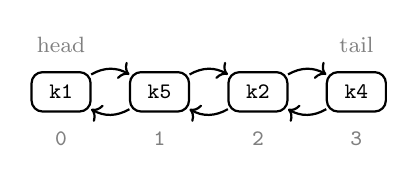
\begin{tikzpicture}
			\node[defaultnode, listnode, scale=0.5] (m1) at (0,0) {};
			\node[defaultnode, listnode, scale=0.5] (m2) at (1.25,0) {};
			\node[defaultnode, listnode, scale=0.5] (m3) at (2.5,0) {};
			\node[defaultnode, listnode, scale=0.5] (m4) at (3.75,0) {};

			\node at (m1) {\footnotesize\texttt{k1}};
			\node at (m2) {\footnotesize\texttt{k5}};
			\node at (m3) {\footnotesize\texttt{k2}};
			\node at (m4) {\footnotesize\texttt{k4}};

			\node[above of =m1, yshift=-4mm, smallgraytext] {head};
			\node[below of =m1, yshift=4mm,  smallgraytext] {\texttt{0}};
			\node[below of =m2, yshift=4mm,  smallgraytext] {\texttt{1}};
			\node[below of =m3, yshift=4mm,  smallgraytext] {\texttt{2}};
			\node[below of =m4, yshift=4mm,  smallgraytext] {\texttt{3}};
			\node[above of =m4, yshift=-4mm, smallgraytext] {tail};

			\draw[->, thick] (m1) edge[bend left] (m2);
			\draw[->, thick] (m2) edge[bend left] (m3);
			\draw[->, thick] (m3) edge[bend left] (m4);
			\draw[<-, thick] (m1) edge[bend right] (m2);
			\draw[<-, thick] (m2) edge[bend right] (m3);
			\draw[<-, thick] (m3) edge[bend right] (m4);

		\end{tikzpicture}
	\end{figure}
\end{frame}

\begin{frame}[fragile]
	A \texttt{List} stores \texttt{ListNode} objects and supports the following operations:\\~\\
	\begin{itemize}
		\item \highlight{\texttt{get}} \\
		      \graytext{returns an object (if it exists)}\\[-1mm]
		      \begin{lstlisting}[style=mypython]
get(idx: Integer) -> Optional[ListNode]
\end{lstlisting}

		\item \highlight{\texttt{insert}} \\
		      \graytext{inserts an object at the specified index}\\[-1mm]
		      \begin{lstlisting}[style=mypython]
insert(Object: Object, idx: Integer) -> Optional[ListNode]
\end{lstlisting}

		\item \highlight{\texttt{delete}} \\
		      \graytext{deletes an object (if it exists)}\\[-1mm]
		      \begin{lstlisting}[style=mypython]
delete(idx: Integer) -> Optional[ListNode]
\end{lstlisting}
	\end{itemize}
\end{frame}

\begin{frame}{Lists (via Doubly Linked Lists)}
	\begin{center}
		\Large \highlight{\texttt{List}} \\[1mm]
		\normalsize\color{gray} (via Doubly Linked Lists)
	\end{center}
\end{frame}

\begin{frame}[fragile]
	\begin{thmboxtop}
		\highlight{\texttt{List}} \\
		\graytext{via Doubly Linked Lists}
		\begin{lstlisting}[style=mypython]
class ListNode:
# attributes
    # the object of this node
    obj: Object
    
    # the previous node
    prev: ListNode
    
    # the next node
    next: ListNode
\end{lstlisting}
	\end{thmboxtop}
\end{frame}

\begin{frame}[fragile]
	\begin{thmboxbot}
		\begin{lstlisting}[style=mypython, firstnumber=last]
class List:
# attributes
    # the first node
    head: ListNode
    
    # the last node
    tail: ListNode
    
    # the number of nodes
    size: Integer

# functions
    ...
\end{lstlisting}
	\end{thmboxbot}
\end{frame}

\begin{frame}
	\begin{center}
		\highlight{\textbf{get}} \\
		\footnotesize\color{gray} \texttt{get(2)}\\
		\normalsize\color{black}
		\begin{figure}
			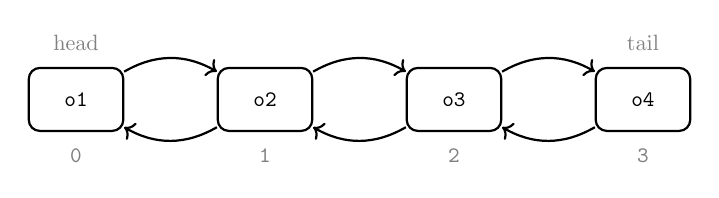
\begin{tikzpicture}[scale=0.8, transform shape]
				\node[defaultnode, listnode] (m1) at (0,0) {\texttt{o1}};
				\node[defaultnode, listnode] (m2) at (3,0) {\texttt{o2}};
				\node[defaultnode, listnode] (m3) at (6,0) {\texttt{o3}};
				\node[defaultnode, listnode] (m4) at (9,0) {\texttt{o4}};

				\node[above of =m1, yshift=-1mm, graytext] {head};
				\node[below of =m1, yshift=1mm,  graytext] {\texttt{0}};
				\node[below of =m2, yshift=1mm,  graytext] {\texttt{1}};
				\node[below of =m3, yshift=1mm,  graytext] {\texttt{2}};
				\node[below of =m4, yshift=1mm,  graytext] {\texttt{3}};
				\node[above of =m4, yshift=-1mm, graytext] {tail};

				\draw[->, thick] (m1) edge[bend left] (m2);
				\draw[->, thick] (m2) edge[bend left] (m3);
				\draw[->, thick] (m3) edge[bend left] (m4);

				\draw[<-, thick] (m1) edge[bend right] (m2);
				\draw[<-, thick] (m2) edge[bend right] (m3);
				\draw[<-, thick] (m3) edge[bend right] (m4);

			\end{tikzpicture}
		\end{figure}
	\end{center}
	\begin{center}
		\graytext{\;}
	\end{center}
\end{frame}


\begin{frame}
	\begin{center}
		\highlight{\textbf{get}} \\
		\footnotesize\color{gray} \texttt{get(2)}\\
		\normalsize\color{black}
		\begin{figure}
			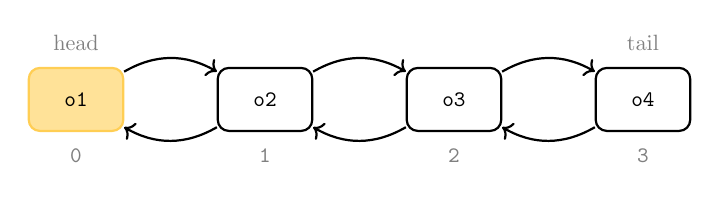
\begin{tikzpicture}[scale=0.8, transform shape]
				\node[newnode, listnode] (m1) at (0,0) {\texttt{o1}};
				\node[defaultnode, listnode] (m2) at (3,0) {\texttt{o2}};
				\node[defaultnode, listnode] (m3) at (6,0) {\texttt{o3}};
				\node[defaultnode, listnode] (m4) at (9,0) {\texttt{o4}};

				\node[above of =m1, yshift=-1mm, graytext] {head};
				\node[below of =m1, yshift=1mm,  graytext] {\texttt{0}};
				\node[below of =m2, yshift=1mm,  graytext] {\texttt{1}};
				\node[below of =m3, yshift=1mm,  graytext] {\texttt{2}};
				\node[below of =m4, yshift=1mm,  graytext] {\texttt{3}};
				\node[above of =m4, yshift=-1mm, graytext] {tail};

				\draw[->, defaultnode, listnode] (m1) edge[bend left] (m2);
				\draw[->, defaultnode, listnode] (m2) edge[bend left] (m3);
				\draw[->, defaultnode, listnode] (m3) edge[bend left] (m4);
				\draw[<-, defaultnode, listnode] (m1) edge[bend right] (m2);
				\draw[<-, defaultnode, listnode] (m2) edge[bend right] (m3);
				\draw[<-, defaultnode, listnode] (m3) edge[bend right] (m4);

			\end{tikzpicture}
		\end{figure}
	\end{center}
	\begin{center}
		\graytext{start at the head}
	\end{center}
\end{frame}

\begin{frame}
	\begin{center}
		\highlight{\textbf{get}} \\
		\footnotesize\color{gray} \texttt{get(2)}\\
		\normalsize\color{black}
		\begin{figure}
			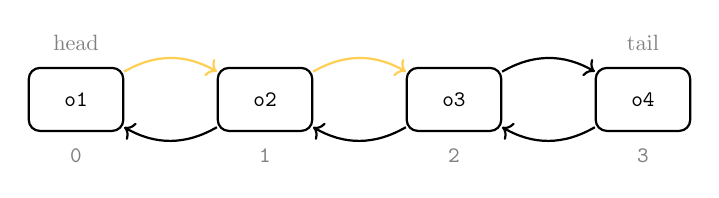
\begin{tikzpicture}[scale=0.8, transform shape]

				\node[defaultnode, listnode] (m1) at (0,0) {\texttt{o1}};
				\node[defaultnode, listnode] (m2) at (3,0) {\texttt{o2}};
				\node[defaultnode, listnode] (m3) at (6,0) {\texttt{o3}};
				\node[defaultnode, listnode] (m4) at (9,0) {\texttt{o4}};

				\node[above of =m1, yshift=-1mm, graytext] {head};
				\node[below of =m1, yshift=1mm,  graytext] {\texttt{0}};
				\node[below of =m2, yshift=1mm,  graytext] {\texttt{1}};
				\node[below of =m3, yshift=1mm,  graytext] {\texttt{2}};
				\node[below of =m4, yshift=1mm,  graytext] {\texttt{3}};
				\node[above of =m4, yshift=-1mm, graytext] {tail};

				\draw[->, newnode, listnode] (m1) edge[bend left] (m2);
				\draw[->, newnode, listnode] (m2) edge[bend left] (m3);
				\draw[->, defaultnode, listnode] (m3) edge[bend left] (m4);
				\draw[<-, defaultnode, listnode] (m1) edge[bend right] (m2);
				\draw[<-, defaultnode, listnode] (m2) edge[bend right] (m3);
				\draw[<-, defaultnode, listnode] (m3) edge[bend right] (m4);

			\end{tikzpicture}
		\end{figure}
	\end{center}
	\begin{center}
		\graytext{traverse the nodes (in order) until the appropriate index is reached}
	\end{center}
\end{frame}

\begin{frame}[fragile]
	\begin{proofbox}
		\begin{lstlisting}[style=mypython]
def get(self: List, idx: Integer) -> Optional[ListNode]:
    curr = self.head
    for _ in range(idx):
        curr = curr.next
        if curr == None:
            break
    return curr
\end{lstlisting}
	\end{proofbox}
\end{frame}

\begin{frame}[fragile]
	\begin{thmboxtop}
		\begin{lstlisting}[style=mypython]
def insert(self: List, idx: Integer, obj: Object) -> Optional[ListNode]:
    if idx < 0 or idx > self.size:
        return None
        
    new = ListNode(obj)
    
    # insert at head
    if idx is 0:
        new.next = self.head
        if self.head:
            self.head.prev = new
        else:
            self.tail = new 
        self.head = new
\end{lstlisting}
	\end{thmboxtop}
\end{frame}

\begin{frame}[fragile]
	\begin{thmboxside}
		\begin{lstlisting}[style=mypython, firstnumber=last]
    # insert at tail
    elif idx is self.size - 1:
        new.prev = self.tail
        if self.tail:
            self.tail.next = new
        else:
            self.head = new
        self.tail = new
\end{lstlisting}
	\end{thmboxside}
\end{frame}

\begin{frame}[fragile]
	\begin{thmboxbot}
		\begin{lstlisting}[style=mypython, firstnumber=last]        
    # insert in middle
    else:
        next = self.get(idx)
        prev = next_node.prev

        new.prev  = prev
        new.next  = next
        prev.next = new
        next.prev = new

    self.size += 1
    return new
\end{lstlisting}
	\end{thmboxbot}
\end{frame}

\begin{frame}[fragile]
	\begin{thmboxtop}
		\begin{lstlisting}[style=mypython]
def delete(self: List, idx: int) -> Optional[ListNode]:
    if idx < 0 or idx >= self.size:
        return None
        
    # delete head
    if idx is 0:
        vic = self.head
        self.head = vic.next
        if self.head:
            self.head.prev = None
        else:
            self.tail = None
\end{lstlisting}
	\end{thmboxtop}
\end{frame}

\begin{frame}[fragile]
	\begin{thmboxside}
		\begin{lstlisting}[style=mypython, firstnumber=last]
    # delete tail
    elif idx is self.size - 1:
        vic = self.tail
        self.tail = vic.prev
        if self.tail:
            self.tail.next = None
        else:
            self.head = None
\end{lstlisting}
	\end{thmboxside}
\end{frame}


\begin{frame}[fragile]
	\begin{thmboxbot}
		\begin{lstlisting}[style=mypython, firstnumber=last]
    # delete middle
    else:
        vic = self.get(idx)
        vic.prev.next = vic.next
        vic.next.prev = vic.prev

    self.size -= 1
    vic.next = None
    
    vic.prev = None
    return vic
\end{lstlisting}
	\end{thmboxbot}
\end{frame}

\begin{frame}[fragile]
	\begin{proofbox}
		\begin{lstlisting}[style=mypython]
def prepend(self: List, obj: Object) -> Optional[ListNode]:
    return self.insert(0, obj)

def append(self: List, obj: Object) -> Optional[ListNode]:
    return self.insert(self.size-1, obj)

def dehead(self: List) -> Optional[ListNode]:
    return self.delete(0)

def detail(self: List) -> Optional[ListNode]:
    return self.delete(self.size-1)
\end{lstlisting}
	\end{proofbox}
\end{frame}

\end{document}